% !TeX spellcheck = en_GB

\subsection{Features and methods}
	
	As in many fields, the frontier between features and methods used for audio tasks have been blurred during the last decades. Usually, a problem is addressed with a pre processing period of the data and then the model or method is implemented. Right now, these two stages are sometimes maintained but also have been mixed or changed depending on how the algorithm used works. In this chapter, we are going to try to explain these difference between features and methods and try to separate them in order to ease its understanding.

\subsubsection{Features}

	In every machine learning or pattern recognition task, for the system to be able to infer and extract conclusions from the input given, it is necessary a pre processing period in order to make some transformations to the data so this can be readable by the model. This stage is known as feature extraction and the goal is to convert the original information into a set of of values or vectors that characterize the data regarding some desired properties \cite{Giannakopoulos2014}.
	
	There are several ways that allow us to perform this processing stage. The most common and basic one consists on extracting features that are really closely related to the original signal which are called \acrfull{lld}  \cite{Amatriain2004}. These are computed by performing some mathematical operations or formulas to the original data that can be considered rudimentary when comparing with other techniques. However, they are really extended and still in use nowadays \cite{Marr1982}. 
	
	\todo{Include small definition short-term features and long-term features?}
	In the audio field, there are two types in which all \acrshort{lld} can be grouped into. One of them is for the features that have been computed by considering the audio signal in its original form in the recording, i.e., in time-domain, that is the reason why they are known as time-domain audio features. The other case refers to those characteristics that are obtained from the signal after been transformed to frequency domain. These are commonly known as frequency-domain or spectral audio features. For the procedure of feature extraction, the signal is usually divided into frames that can be overlapped by using a sliding window, so the calculations are done per frame, obtaining a final matrix with size $number\ of\ frames \times number\ of\ features$ \cite{Giannakopoulos2014}. It must be taken into account that the final application of the whole system is going to be fundamental at the time of deciding which features must be computed. For example, not the same features are used for speech recognition than for musical information retrieval. In table \ref{table:6}, a summary of most used time and spectral features is included.
	
	% Table of time domain features
	\begin{table}[h!]
		\begin{center}
			\centering
			\begin{tabular}{|| m{9em} | m{24em} ||}
				\hline
				\begin{center}\textbf{Feature}\end{center}& \begin{center}\textbf{Description}\end{center} \\
				\hline\hline
				\multicolumn{2}{||c||}{\textbf{Time}} \\
				\hline
				Energy Entropy & It is a useful to detect sudden changes from the energy of a signal. To calculate this value for a certain subframe, it is necessary to first compute the normalized energy of the subframe with respect to all the frames energy \cite{Giannakopoulos2006}. \\
				\hline
				Short time energy & It is the energy for a short segment of signal. It is normally used in speech tasks in order to identify voiced form non-voiced fragments \cite{Garcia-Gomez2016}. \\
				\hline
				\acrfull{zcr} & This can be defined as the number of times the amplitude of the signal crosses the zero line, i.e., changes from negative to positive. It is computed by the number of zero-crossings by the amount of samples in the frame \cite{Giannakopoulos2006}. \\
				\hline
				\multicolumn{2}{||c||}{\textbf{Frequency}} \\
				\hline
				\acrfull{sf} & It is computed to measure the spectral changes between two successive frames. To do so, the difference is calculated through their squared spectra coefficients normalized \cite{Giannakopoulos2006}. \\
				\hline
				Spectral Rolloff & This represents the skewness of the shape of the spectrum by given the frequency below which a concrete percentage of the magnitude distribution of the frequency transform is concentrated \cite{Garcia-Gomez2016}. \\
				\hline
				\acrfull{sc} & This is a measure related to the spectral position. It is defined as the center of gravity of the spectrum, i.e., \doubt{it indicates how high the spectrum values are on average} \cite{Giannakopoulos2006}. \\
				\hline
				\acrshort{mfcc} & It is a feature that it is widely used and it has given such good results, mainly within the speech recognition field because it interprets the frequency bands in a very similar way to human perception. It is computed from the \acrshort{stft}.\cite{Garcia-Gomez2016}. \doubt{A detailed explanation can be found in appendix \ref{}}. \\
				\hline
			\end{tabular}
		\end{center}
		\caption{Time-domain and spectral audio features}
		\label{table:6}
	\end{table}

	Then, a typical procedure would first divide the signal into frames and performed the desired mathematical and statistical transformations to obtain a \acrshort{lld} vector per sample in order to pass these input data to a statistical model that will be trained with the objective of summarizing the properties of the signals and develop a classification rule so as to be able to assign a faithful category to a new unlabelled observation \cite{Stowell2015}.
	
	In some cases, the mentioned descriptors are not enough to model data, just because they cannot achieve an enough meaningful representation of the original information for the system to learn from it. Also, as mentioned above, the selection process of this type of features plays a significant role in the final output so that the criteria of the designer could be considered a limitation for the classification task \cite{Grill2012}. For this reason, a new strategy of addressing feature extraction process has appeared based on the idea of finding more specialized properties by using specific engineering algorithms that explores the given data in order to find non-human recognizable patterns. The techniques that allow to perform this task are usually called automated feature generation algorithms \cite{Pachet2009}.
	
	In order to compute these high-level features, there is not just one standardized machine model that allow to compute them all in a particular form. The calculation method, nevertheless, differs from one approach to another. One example could be the combination of low-level data with high-level semantic descriptors that consists on the inference of diverse musical dimensions by using support vector machines so as to find similarities among music genres. Particularly, they consider the output probabilities of the \acrshort{svm} classifier as a high-level feature space in which the distance between samples from different classes can be measured \cite{Bogdanov2011}. Other application example could be building high-level feature detectors for image recognition by using unlabelled data to feed a \acrshort{nn} model \cite{Le2013}. 
	
\subsubsection{Classification models}
	
	Several algorithms have been designed in order to perform the classification task by finding data patterns from input data features. \doubt{We are going to include a small explanation of some of the most common used in the literature and go deeper in those we have used}. Some of the most common and base methods to tackle the classification task are \acrshort{knn}, \acrshort{svm} and also \acrshort{gmm} \cite{Fu2011}.
	
	In the case of \acrfull{knn}, if there is a set of samples ${x_1, ..., x_n}$ that belong to a metric space $X$ whose labels are ${\theta_1, ..., \theta_n}$ respectively, if a new sample $x$ comes in, it will be categorized by following a majority vote process of the nearest neighbours considering the distance in the space $X$. A \doubt{engagement relationship} must exist in the number of nearest neighbours since it is desirable to be large for the voting process to have more participants and minimize the probability of misclassification and, also, a small value with respect to the total number of samples so the nearest points are close enough to the new observation \cite{Cover1967}. \todo{Complete with example in the ASC or AEDC approaches}
	
	In the case of \acrfull{gmm}, it is a soft clustering method. It is commonly used to derive global statistical properties from the feature vectors of the sample data. Specifically, considering $K$ clusters, it defines a group of feature vectors from training data and belonging to a certain category $q$ modelled as a multivariate normal distribution $N(\mu_k, \Sigma_k)$ that is weighted by the probability $w_k$ of a particular of a certain observation to belong to cluster $k$. After learning a global model for the training data $M_q={w_k, \mu_k, \Sigma_k}$, a new observation will be categorized by applying the maximum likelihood criterion \cite{Stowell2015}.
	
	However, the one that have been generally more successful is the \acrfull{svm} classifier. There have been published plenty of works that use this technique for audio classification tasks \cite{Jiang2005} \cite{Geiger2013} \cite{Barchiesi2015}. It is commonly known to be a binary classifier but, nowadays, there have been some implementations that allow to use it in a multiclass problem. This algorithm makes the classification by taking into account the two observations that are more likely to be misclassified and draw a hyperplane as the optimal frontier between the two classes \cite{Fu2011}. Since this technique has been used for the experiments in this work, a more detailed explanation is included in section \ref{section:models}.
	
	As a final kind of method, it should be mentioned all the techniques or algorithms that have been developed based on the idea of \acrfull{ann}. This concept was animated by human biology and how the neurons communicate among them inside a brain in order to interpret the input data the human senses collect. 
	
	The \acrshort{ann} intention is exactly to transform input data into a desired output space so it can understandable by a machine. A basic architecture is usually composed by an \textit{input layer} of neurons, a certain number of \textit{hidden layers} and an \textit{output layer}. The model receives some input, typically a feature vector, and pass it trough the hidden layers in order to perform some transformations. The neurons of a layer are completely connected to the neurons of the next layer but neurons in the same layer are totally independent. For this case, we can say that they are \acrfull{fc} layers. Finally, the output layer gives the final outcome of the network \cite{Kwon2011}. This is just the basic and initial nature of the idea but it was implemented in many different ways depending on the input data and the desired task.
	
	\todo{Include image of FCC?}
	
	
	% !TeX spellcheck = en_GB
% CNN explanation

\label{section:cnn}

	One of the most explored implementations is the one related to \acrfull{cnn}. This maintain the basic idea of receiving some inputs and apply a dot product operation to them before subject the data to a non-linear function but with the difference that input data are expected to be images \cite{Karpathy2016}. The architecture of a \acrlong{convnet} is based on the organization of the Visual Cortex in the human brain. This means that single neurons responds to some stimuli only in a certain region of the visual field, the Receptive Field. Then, a collection of these fields overlap with each other so as to cover the full visual space \cite{Saha2018}.
	
	About the input data, it is introduced as a matrix instead of as a row vector. Then, the architecture of the layers adapt to the fact that input data are images. They do not consist of a single row of neurons, but they have a shape constituted by three dimensions: heigh, width and depth \cite{Karpathy2016} \todo{include image?}. In this way, the net can capture the spatial and temporal relations present in an image by applying some filter functions. With this construction, the model can be trained with a smaller number of parameters and also reuse the weights.
	
	A \acrlong{convnet} can be described as a sequence of layers in which every layer converts a volume of activation results from the previous layer to another by computing a differentiable function. The architecture of a \acrshort{cnn} is always composed by three type of distinguishable layers which are \textit{Convolutional}, \textit{Pooling} and \textit{\acrlong{fc}}. A normal architecture will follow the next succession of layers \cite{Karpathy2016}:
	
	\begin{itemize}
		\item INPUT: this represents the image at the entrance of the whole model. It commonly is a 3\acrshort{d} matrix , one dimension per channel of colour, and contains the values of the original pixels.
		\item CONVOLUTIONAL: considering the neurons that are connected to a region of the input image, this layer computes their output by performing a dot product between the weights and the value of the pixels. The depth of the resulting data will coincide with the number of filters used.
		\item POOL: this performs a fixed operation that consists of a downsampling of the spatial dimension. It typically reduces by half the height and the width of the input image.
		\item \acrshort{fc}: this is the final layer which gives the output of the whole net. It is a vector-shape layer and is completely connected to the previous layer. In a classification task the number of neurons matches the amount of classes of the problem.
	\end{itemize}
	
	Note that this list represents the order of the layers in the architecture, however, the number of layers of each type vary depending on how the model is designed and how deep it is desired to be. For example, some examples of deep architectures can be found later in section \ref{subsection:vgg}, in table \ref{table:3}.
	
	With this building, a \acrlong{convnet} passes the information of the pixels layer by layer while reducing the input images in a way that is much easier to process. This is performed without missing any feature since all of them are essential to compute a good prediction outcome.
	
	In the convolutional layer, a convolution operation is performed for each small region of the input image. The element that carries out this operation is called \textit{kernel} or \textit{filter}. This partial region that the kernel covers in the input data is set by deciding the height and the width as a designing parameter. About the depth, it must match the depth of the input data so the filter can slide trough the image along its 2\acrshort{d} and obtaining the results of the convolution operation by computing between the pixels inside the region and the values of the filter. An example can be observed in figure \ref{fig:mesh11}. For each filter, a 2\acrshort{d} activation map is obtained after subjected the result of the convolution to a non-linear operation as the \acrfull{relu} function. Finally, we will pack all these in a unique volume that will consists in the output of the convolutional layer \cite{Karpathy2016}. For example, if we have a number of 64 filters, we will get then a group of 64 2\acrshort{d} activation maps that will be the input of the next layer. Traditionally, it was the first convolutional layer the one that was responsible of capturing low-level features related to edges or colours in the image. The upper layers were the ones in charge of extracting high-level features so the network was able to understand the image similar to how the humans do \cite{Saha2018}.
	
	\begin{figure}[ht]
		\centering
		\captionsetup{justification=centering}
		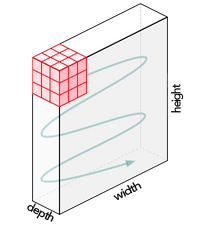
\includegraphics[scale=0.6]{movement-of-kernel}
		\caption{Movement of the kernel represented as a red block along the width and the height of the original input image. It is clear that it occupies the whole depth of the input image. The arrow indicates an approximation of the movement that the filter follows \cite{Saha2018}.}
		\label{fig:mesh11}
	\end{figure}

	We have included how the input interacts with the convolutional layer and also introduced the concept of depth of the resulting volume. However, it is needed to explain the how the total size of this output is computed and what it depends on. There are three main parameters that play a role in this decision: \textit{depth}, \textit{stride} and the \textit{zero-padding} \cite{Karpathy2016}.
	
	\begin{itemize}
		\item DEPTH: it is a hyperparameter that corresponds to the amount of kernels used in the convolutional layer when learning from the input.  The set of neurons that extent through the depth dimension operating in the same region is called depth column. This is the previous mentioned red block shown in figure \ref{fig:mesh11}.
		\item STRIDE: this indicates the displacement of the sliding filter along the image. If it has a value of 1 (non-strided), this means that the kernel will shift a position of one pixel along the width. When it is set to 2, then it moves two pixels. It rarely has values greater than 2. The moving process consists on the filter going from right to left with a hop determined by the stride value. When the right margin is reached, then it jumps to the beginning of the next row from the left margin and repeats the process in the same way until the image is completed \cite{Saha2018}. The bigger the stride, the smaller the size of the output volume.
		\item ZERO-PADDING: this is also called just \textit{padding}. It consists on adding zeros to the borders of the image. What is a hyperparameter in design is the size of this padding. This allows to control the width and height of the output volume so we can keep it the same through the different layers. When it is indicate a "valid padding", it means that no padding is added and the output size will be reduced. If we indicate "same padding", then it has a value of 1 and means that the resulting volume will have the size of the input \cite{Keras}.
	\end{itemize}

	As shown below, the total size of the obtained volume, $D$, can be computed as function of the input size, $W$, the spatial 2\acrshort{d} dimensions of the convolutional filter, $F$, the stride of the filters shifting, $S$,  and the amount of padding in the zero-padding, $P$ \cite{Karpathy2016}. 
	
	\[ D = \frac{W - F + 2P}{S} + 1 \]
	
	The convolutional layers can be grouped all together, one after another, but they are usually interpolated by what it has been previously defined as \textit{pooling} layer. This habit has the objective of reducing the the width and the height of the resulting volumes in a progressive manner in order to decrease the total number of training parameters and control the computational cost, and, therefore to avoid overfitting \cite{Karpathy2016} \todo{Include definition of overfitting or just cite it}. There can be performed two types of pooling operation: the max-pooling or the average-pooling. The former just returns the maximum value from the portion of the image where the filter is placed. The latter, computes the average of all the values in this portion \cite{Saha2018}. The pooling layer acts in an independent way on every input depth level. 
	
	Two hyperparameters are needed in order to configure the spatial portion in which the pooling is computed: the  filter size, related to length of height and width, and the stride. However, for this operation zero parameters are introduce since it consists on a fixed operation over the input data. In figure \ref{fig:mesh12}, it is shown how the max-pooling operation is performed \cite{Karpathy2016}. 
	
	\begin{figure}[ht]
		\centering
		\captionsetup{justification=centering}
		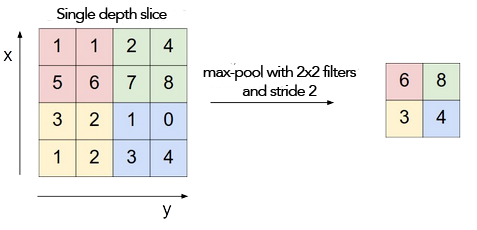
\includegraphics[scale=0.7]{max-pooling}
		\caption{Max-pooling operation with a filter size of 2 and a stride of 2 for a single depth filter. Each colour represents a the action portion for each operation \cite{Karpathy2016}}
		\label{fig:mesh12}
	\end{figure}
	
	Together a convolutional layer and a pooling layer constitute a complete layer structure typical in a \acrlong{convnet}. The number of these complete layers can vary depending on the design and the task needs. These represent the main core of the network before passing to the last layers and calculating the final output \cite{Saha2018}.
	
	For the final step, a common way of acting is to apply some non-linear activations in order to learn from the high-level features resulted from the output volume of the last convolutional layer. This takes place in the \acrlong{fc} layers ending the model. This part has the shape of a Fully-Connected layer, as the one described in the basic model of \acrshort{ann}. To make the weights from the convolutional layers available to feed this last part of the model, it is necessary to flatten the output volume and obtain a column vector. The learning process is possible due to a backpropagation operation performed in every epoch of training. As a total output, the values that represent the classification of the different samples into one or another category are obtained \cite{Saha2018}. A common classification technique is the one called \textit{Softmax}. This normalizes the result of the previous \acrshort{fc} layer into a vector whose values follow a distribution that total sum results in 1. This type of output is called \textit{soft predictions} and represent the probability for each sample of belonging to a category in the classification \cite{Mahmood2018}. However, there exists other activation functions that can compute the classification output in other ways. 
	
	In figure \ref{fig:mesh13} an scheme of a common \acrlong{cnn} is shown. This takes an input image, compute the features along three groups of convolutional layer plus max-pooling and, finally, includes three \acrlong{fc} layers, being the last one a softmax function layer with as many neurons as classes that gives the soft predictions for this image of belonging to each class.
	
	\begin{figure}[ht]
		\centering
		\captionsetup{justification=centering}
		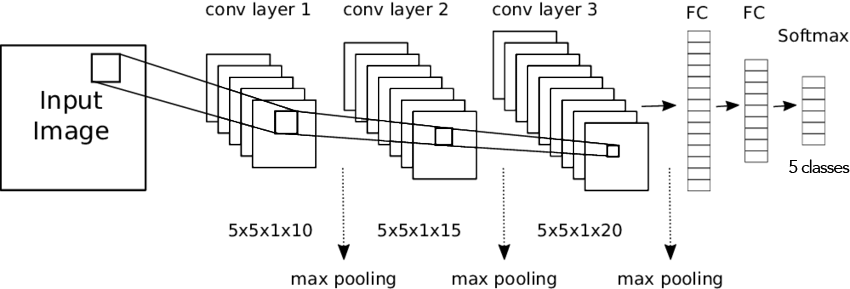
\includegraphics[scale=0.4]{cnn}
		\caption{Representation of a typical CNN model \cite{Hinz2016}}
		\label{fig:mesh13}
	\end{figure}

	\acrfull{cnn} were originally designed to work with images but they have been applied to other fields as audio. An image can be defined as a matrix of values, i.e. pixels, in two or three dimensions, so the only prerequisite to use a \acrshort{cnn} is to have the input data in this form. For audio researching, it has been commonly used the log-scaled mel spectrogram, that is a way of representing audio in a scale different than frequency that is more similar to humans perception. It has been used in plenty of works with \acrshort{cnn} and also combined with other techniques \cite{Salamon2017} \cite{Piczak2015} \cite{Kumar2017}.
	
	
	

	

	
	
	
	
	
	
	% !TeX spellcheck = en_GB

\subsection{\acrlong{rnn} and \acrlong{lstm}}

	Human learning does not happen at each moment independently in the sense that every time something new is learned, it depends on the previous knowledge in order to interpret it. This can also be explained by saying that our understanding is persistence.
	
	Traditionally, \acrlong{ann} are not able to act in this way. They \doubt{cannot use the time} as a property to infer conclusions or predictions from the previous instances that belong to a sequence of data. To address this task \acrfull{rnn} have been developed, so they can take information and make it persistent. In figure \ref{fig:mesh39}, it is shown a block of a \acrshort{rnn} in which the network, \textit{A}, is fed with an input \textit{x\textsubscript{t}} that is actually a sequence of data. The output is the value \textit{h\textsubscript{t}}. An inner loop takes the information from the outcome and pass to the input for the next learning step. This can be easily seen in the unrolled part of the right, how the information flows from one element to the next one \cite{Olah2015}. 
	
	\begin{figure}[h]
		\centering
		\captionsetup{justification=centering}
		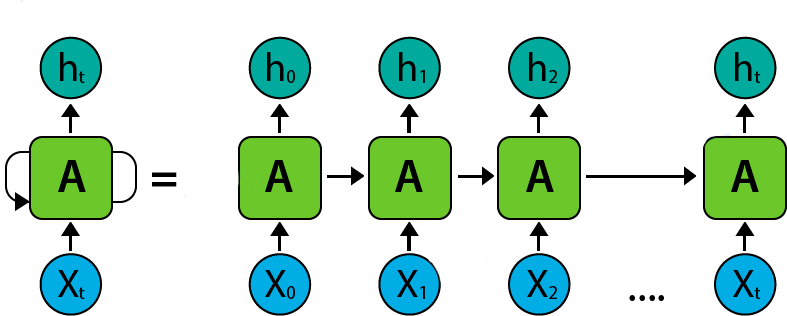
\includegraphics[scale=0.35]{rnn}
		\caption{Scheme or a recurrent neural network about how the loop works }
		\label{fig:mesh39}
	\end{figure}

	This type of networks has became the standard when dealing with sequential data. They have been applied in many tasks, such as language modelling, speech recognition, translation, etc. However, the most simple approach present a problem when the information that must be considering when long-term dependencies. For example, if the task consists of predicting a new instance based on the previous ones in a not really long sequence in which the dependency resides on close instances, normal \acrshort{rnn} can be used and work in the way explained above. When the distance inside the sequence between the predicted element and the ones with the important information that this new one depends on is too large, the network cannot learn this connection \cite{Olah2015}. 
	
	\begin{figure}[h]
		\centering
		\captionsetup{justification=centering}
		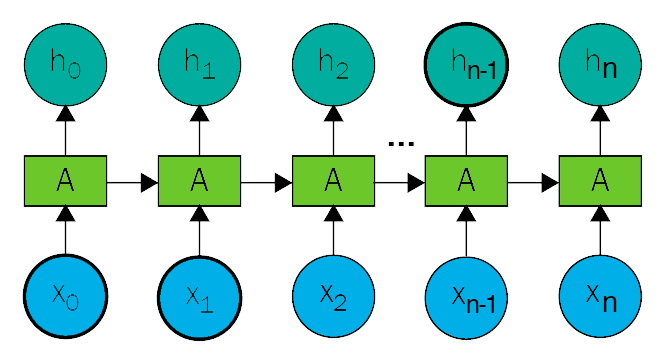
\includegraphics[scale=0.35]{long-term-dependencies}
		\caption{Example of long-term dependencies situation. If the predicted output h\textsubscript{n-1} depends on x\textsubscript{0} and x\textsubscript{1}, the vanishing gradient problem may appear.}
		\label{fig:mesh40}
	\end{figure}
	
	This happens due to the value of the gradients becomes very small during the backpropagation in the learning process. Once the loss function for the new predicted output is calculated, this must be propagated through the rest of the network in order to update the weights. In a typical neural network model, \doubt{the neurons that get updated are those from the hidden layer directly previous to the output one}, but, since the data is a sequence, the neurons from all the earlier layers must be updated as well. The actual problem appears when renovating the value of the weights through time, i.e. updating the weights used to connect the hidden layers in the unrolled temporal loop. So, if the value of the gradient becomes very small the updating process start to be null when finding the new values of the weights and the model stop learning. This is known as the vanishing gradient problem \cite{SuperDataScienceTeam2018}.
	
	As a solution, a new type of \acrshort{rnn} was developed and named as \acrfull{lstm} networks. These can be defined as a recurrent network that can learn long-term dependencies, so the vanishing gradient problem is not an issue for these models. Nowadays, they are widely used in several fields, since they can remember information along long periods \cite{Olah2015}. The main structure along is the same shown above in figure \ref{fig:mesh39}. The difference from the way of working in a common \acrshort{rnn} is the inner architecture in the neural network. In \acrshort{lstm}, the \textit{A} modules are defined as shown in figure \ref{fig:mesh41}. The notation used is as follows: the rectangles denotes a neural network layer, the circle shapes refer to point-wise operations and the arrows means vector transferring.
	
	\begin{figure}
		\centering
		\captionsetup{justification=centering}
		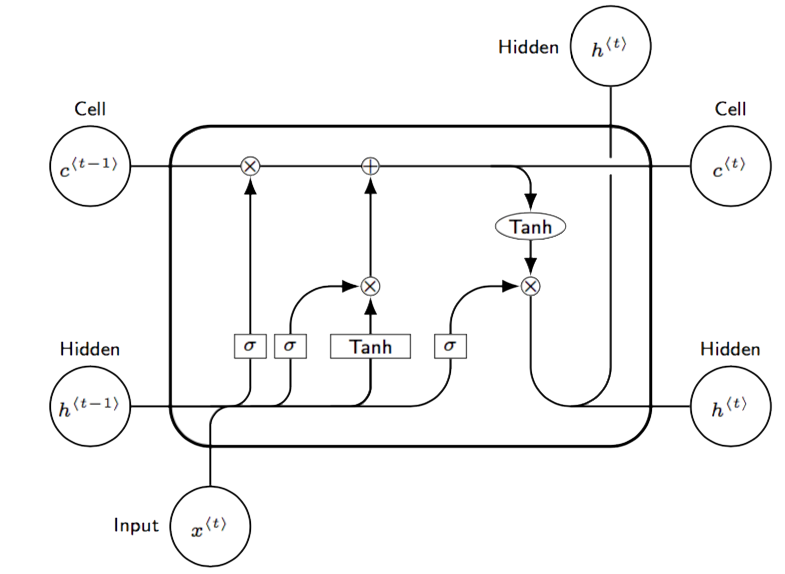
\includegraphics[scale=0.29]{lstm-module}
		\caption{LSTM module with the representation of the different operations that take place inside of it}
		\label{fig:mesh41}
	\end{figure}

	The main concept of a \acrshort{lstm} network resides on its cell state and the different gates. The cell state, represented in the diagram by the upper arrow, is the one in charge of transferring information all the way through the chain of modules. It can be thought as the memory of the whole network. Its objective is to just carry information considered relevant for the model. This way is how the \acrshort{lstm} brings the information from the first layers to the last ones without suffering the vanishing gradient problem. The content of the cell state is modified by the point-wise operations that acts by following the gates criteria. These are in fact neural networks that has the goal of deciding which information can be treated as relevant and so added to cell state. This process can be understood as a learning/forgetting stage \cite{Nguyen2018}. 
	
	In order to understanding how this process works, we are going the interaction of the different gates in the learning stage.

	\begin{wrapfigure}{l}{0.26\textwidth}
		\centering
		\captionsetup{justification=centering}
		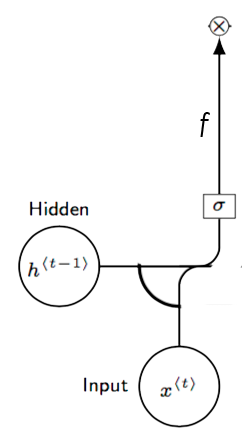
\includegraphics[scale=0.25]{lstm-forget-gate}
		\caption{Step 1. Forget gate}
		\label{fig:mesh42}
	\end{wrapfigure}

	The first step is performed by what is called the \textit{forget gate} layer. It must decide which information must be included in the cell state that travels through the time chain. This is way the layer contains a sigmoid function that outputs values between  0 and 1, in which  0 means dropping the information in the previous cell state and 1 implies to keep it. As shown in figure \ref{fig:mesh42}, this is done by paying attention to the hidden state which is the output of the previous module, \textit{h\textsuperscript{<t-1>}}, and the input of the current one, \textit{x\textsuperscript{<t>}} \cite{Nguyen2018}. The resulting function $f$ is defined as follows, where $W_{f}$ are the weights of the \acrshort{rnn} and $b_{f}$ the bias.
	\[
	\ f = \sigma(W_{f}[h^{t-1}, x^{t}] + b_{f})
	\]
	
	\begin{wrapfigure}{r}{0.3\textwidth}
		\centering
		\captionsetup{justification=centering}
		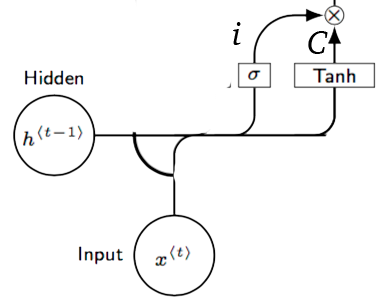
\includegraphics[scale=0.27]{lstm-input-gate}
		\caption{Step 2. Input gate}
		\label{fig:mesh43}
	\end{wrapfigure}
	
	Next, the decision about what information from the current input \textit{x\textsuperscript{<t>}} must be taken to the cell state is performed. The gate that computes this operation receives the name of \textit{input gate}. This part can be divided into two different steps. First, the previous hidden state,\textit{x\textsuperscript{<t-1>}} ,and the current input feed a \acrshort{rnn} with a sigmoid for the activation function, which takes the decision of \doubt{which values must be updated} by converting them into a range limited by 0 and 1. This result denotes the importance of the value, being 0 non-important and 1, important. Then, also \textit{h\textsuperscript{<t-1>}} and \textit{x\textsuperscript{<t>}} are used as input for the \acrshort{tanh} layer so the values are mapped between -1 and 1. This last activation function is included in order to \doubt{avoid the vanishing gradient problem previously mentioned, since a function whose second derivative takes more time to tend to zero is needed}. Finally, both outputs are multiplied before the updating process in the cell state \cite{Nguyen2018}. The equations for the output of each \acrshort{rnn} module are included below, where $W$ and $b$ denotes the weights and bias for each layer \cite{Olah2015}.
	\[ i = \sigma(W_{i}[h^{t-1}, x^{t}] + b_{i}) \]
	\[ C = \tanh(W_{C}[h^{t-1}, x^{t}] + b_{C}) \]
	
	In the step 3, the output of the multiplication from the input gate layer and the output $f$ of the sigmoid function from the forget gate, modify the old cell state from the previous module, \textit{c\textsuperscript{<t-1>}}, so it can be updated. For the outcome of the step 1, a point-wise multiplication is performed, $f * C^{<t-1>}$. Then, to the output of this operation is added the resulting product of the input gate, $i * C$. This two operations can be translated as a forgetting and a learning stage. First, the values the forget gate decided to remove from the cell state are actually forgotten. Then, it must learn the new values belonging to the current input also weighted by their importance, what denotes how much the state values are going to be updated \cite{Olah2015}. The new cell state expression $c^{t}$ is included below and the process is shown in figure \ref{fig:mesh44}.
	
	\begin{wrapfigure}{l}{0.4\textwidth}
		\centering
		\captionsetup{justification=centering}
		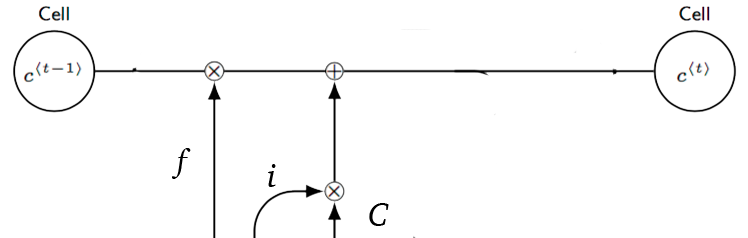
\includegraphics[width=\linewidth]{lstm-cell-state}
		\vspace{-10pt}
		\caption{Step 3. Update cell state}
		\label{fig:mesh44}
	\end{wrapfigure}
	
	
	\[c^{<t>} = f * C^{<t-1>} + i * C\]
	
				
	Finally, the last step of the module corresponds to the \textit{output gate}. This has the function of deciding how the next hidden state is going to be like. First, \textit{x\textsuperscript{<t>}} and \textit{h\textsuperscript{<t-1>}} are used as input for a layer with a sigmoid activation function and the output $o$ is obtained. Also, the cell state \textit{c\textsuperscript{<t>}} feeds a point-wise \acrshort{tanh} so its values are clipped between -1 and 1. Both outputs are multiplied. The $o$ result decides what values form the current input must be kept in the future hidden state,\textit{h\textsuperscript{<t>}}. The actual output of the module is the hidden state. It also transports the relevant information updated together with the cell state to the next network. The outputs $o$ and $h^{t}$ can be defined as shown below. Also, in figure \ref{fig:mesh45}, the stage of this last part is included.
		
	\begin{figure}{h}
		\centering
		\captionsetup{justification=centering}
		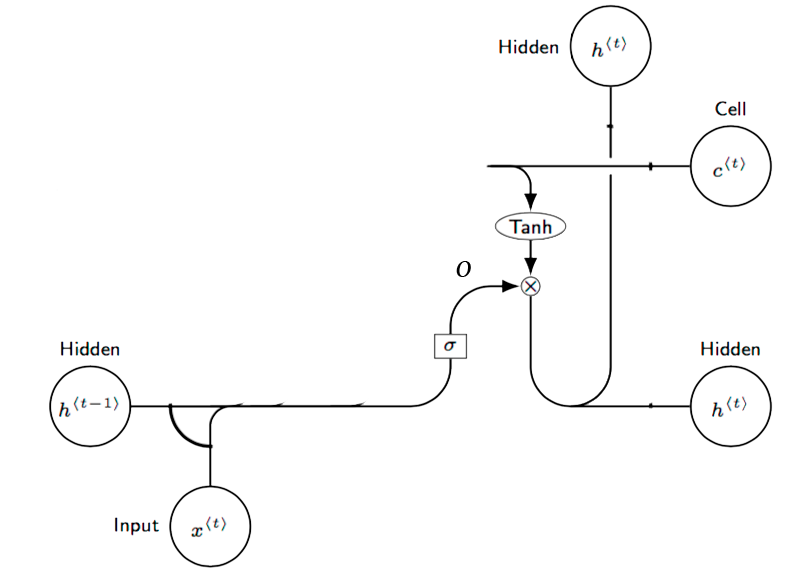
\includegraphics[scale=0.25]{lstm-output-gate}
		\caption{Step 3. Output gate}
		\label{fig:mesh45}
	\end{figure}
	
	\[ o = \sigma(W_{o}[h^{<t-1>, x^{t}}] + b_{o}) \]
	\[ h^{<t>} = o * \tanh(C) \]
	
	
	
	
	

	
	
	
	

	
	
	
	
	
	
	
	